\documentclass{article}
\usepackage{graphicx}
\usepackage{listings}
\usepackage{hyperref}
\usepackage{pdfpages}
\usepackage{float}
\makeatletter
\newcommand\urlfootnote@[1]{\footnote{\url@{#1}}}
\DeclareRobustCommand{\urlfootnote}{\hyper@normalise\urlfootnote@}
\makeatother

\begin{document}
\title{Neural Networks Assignment 1}
\author{Oliver Scherf\\Matthias Mueller-Brockhausen}
\maketitle
\lstset{
  basicstyle=\ttfamily,
  keywordstyle=\bfseries,
  language=Java,
  frame=single,
  aboveskip=11pt,
  belowskip=11pt,
  breaklines=true,
  breakatwhitespace=false,
  showspaces=false,
  showstringspaces=false,
  numbers=left,
  stepnumber=1,    
  firstnumber=1,
  numberfirstline=true
}
\section{Excercise 1: Image Distance}
\label{a1}
Most Difficult to seperate: \[ 7 \rightarrow 9; 4 \rightarrow 9; 3 \rightarrow 5; 9 \rightarrow 8\]

This is the table for our cloud distances.
The lowest and hence most similar values we found were 5.43, 6.01, 6.12 and 6.4.
These values were for classifying 7 to 9, 4 to 9, 3 to 5 and 9 to 8.
This does make sense given that a 9 can be, if written by hand, sometimes hard to distinguish from a 7, 4 or 5.


\section{Excercise 2}
\subsection{Confusion Matrix Training and Test Set}
%Which digits were most difficult to classify correctly?%
%Describe your findings. Compare performance of your classifier on the train and test sets. %
The confusion matrices can be found in Figure \ref{fig:cftrain} for the training set and in Figure \ref{fig:cftest} for the testing set.
For the training set (Figure \ref{fig:cftrain}) the number 5 and 4 are most difficult to be classified. Very close in error rates and also harder to identify are 0, 2, 5, 6, 7, 8, 9. The only number with full accuracy is 1. This is quite surprising given that 1 and 7 sometimes look quite alike.

For the testing set (Figure \ref{fig:cftest}) the number 2 is most difficult to classify. Followed by 8, 0, 9, 7 and 3. Also here we have full accuracy for the digit 1.


\begin{figure}[H]
\centering
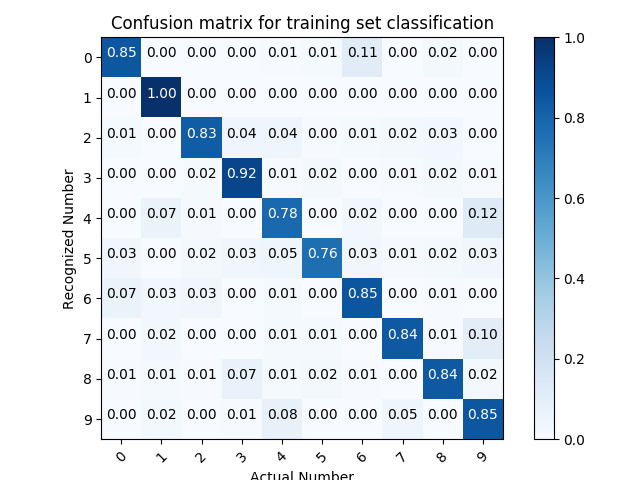
\includegraphics[width=0.9\linewidth]{img/cftrain.png}
\caption{Confusion Matrix visualized for Training Set}
\label{fig:cftrain}
\end{figure}
\begin{figure}[H]
\centering
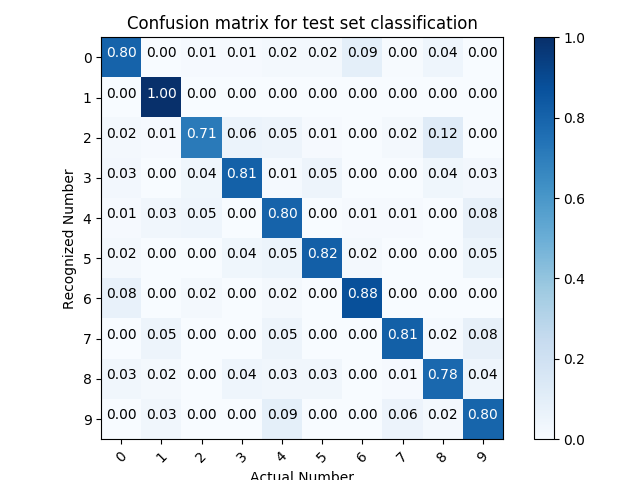
\includegraphics[width=0.9\linewidth]{img/cftest.png}
\caption{Confusion Matrix visualized for Training Set}
\label{fig:cftest}
\end{figure}

\subsection{Comparison to expectations from A1}
%How do the results compare to the observations you’ve made in Step 1? How would you explain it?%
When comparing our findings with the expectations build up in Excercise 1 (see Section \ref{a1}) the occured misclassifications are quite different, given that in the Test Set 2 was most difficulty to classify but that wasn't even in scope of being a problem according to the results of Section \ref{a1}.
This difference could be explained by the amount of actual sample numbers per digit in the classified set.

\subsection{Evaluating different performance measures}
%Which distance measure provides best results (on the test set)?%
In order to determine which distance provider fairs out the best, we applied each of them, and measured the amount of correctly classified occurrences.\newline
Doing so provided us with the following results (sorted by best first):
\begin{itemize}
\item Euclidian / L2: 80.4\% $\rightarrow$ 804 / 1000 correctly classified
\item Cosine 79.9\% $\rightarrow$ 799 / 1000 correctly classified
\item Cityblock / Manhattan / L1: 72.1\% $\rightarrow$ 721 / 1000 correctly classified
\end{itemize}

\section{Excercise 3: Bayesian Classification}
%Which feature do you want to use to discriminate between the two classes?%
\subsection{Choices}
We will be comparing the digits \textbf{1} and \textbf{8}.
To compare these two numbers we will use the ratio between the upper half of the image and the lower half of the image. We decided to use this feature because it is dead simple to extract, but should be different enough to distinguish a 1 and 8.


%Implement your feature, apply it to the training data, discretize it and create corresponding histograms.%
\subsection{Histogram}
The histogram can be seen in Figure \ref{fig:histogram}.
From the histogram we concluded that around 1.10 and 1.15 might be a good point to finish the distinction.

%What accuracy have you achieved?%
We achieved an accuracy of 56.338\%, which is given the simple classifier not too bad. This bad quality was already forseable given that there are quite many 8s with a value below 1.10. (120 correctly classified out of 213)
\begin{figure}[H]
\centering
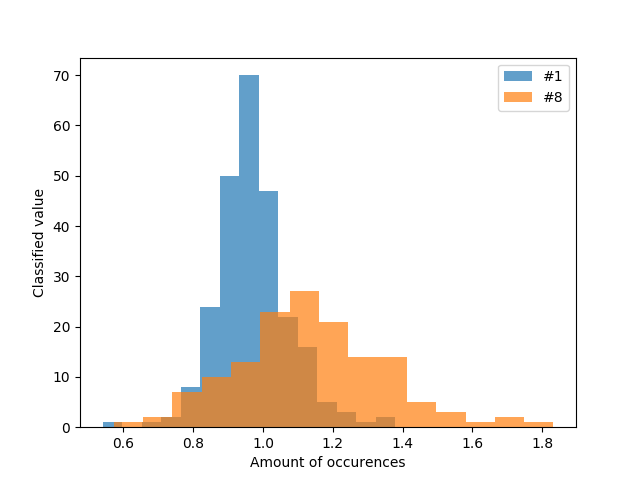
\includegraphics[width=0.9\linewidth]{img/histogram.png}
\caption{Histogram for identifying Digit 1 and Digit 8 based on our selected feature.}
\label{fig:histogram}
\end{figure}

\section{Exercise 4: Multiclass Perceptron}


\end{document}